% Use only LaTeX2e, calling the article.cls class and 12-point type.

\documentclass[12pt]{article}
\usepackage[hyphens]{url}
\usepackage{graphicx}
\usepackage{subcaption}
\usepackage[margin=1in]{geometry}
\usepackage[shortlabels]{enumitem}
\usepackage{adjustbox}
\usepackage{caption}
\usepackage{pgf,tikz}
\usetikzlibrary{shapes.geometric, arrows}
\usepackage{multicol}
\usepackage{amsmath}
\usepackage{tabularx}
\usepackage{graphicx}
\usepackage{subcaption}
\usepackage{wrapfig}


% Users of the {thebibliography} environment or BibTeX should use the
% scicite.sty package, downloadable from *Science* at
% www.sciencemag.org/about/authors/prep/TeX_help/ .
% This package should properly format in-text
% reference calls and reference-list numbers.

\usepackage{scicite}

% Use times if you have the font installed; otherwise, comment out the
% following line.

\usepackage{times}
\usepackage{indentfirst}


\graphicspath{ {Images/} }


% The preamble here sets up a lot of new/revised commands and
% environments.  It's annoying, but please do *not* try to strip these
% out into a separate .sty file (which could lead to the loss of some
% information when we convert the file to other formats).  Instead, keep
% them in the preamble of your main LaTeX source file.



% The following parameters seem to provide a reasonable page setup.

\topmargin 0.0cm
\oddsidemargin 0.2cm
\textwidth 16cm 
\textheight 21cm
\footskip 1.0cm


%The next command sets up an environment for the abstract to your paper.


\newcommand\keywords{\textit{Keywords: } }{}


% If your reference list includes text notes as well as references,
% include the following line; otherwise, comment it out.

\renewcommand\refname{References and Notes}

% The following lines set up an environment for the last note in the
% reference list, which commonly includes acknowledgments of funding,
% help, etc.  It's intended for users of BibTeX or the {thebibliography}
% environment.  Users who are hand-coding their references at the end
% using a list environment such as {enumerate} can simply add another
% item at the end, and it will be numbered automatically.

\newcounter{lastnote}
\newenvironment{scilastnote}{%
\setcounter{lastnote}{\value{enumiv}}%
\addtocounter{lastnote}{+1}%
\begin{list}%
{\arabic{lastnote}.}
{\setlength{\leftmargin}{.22in}}
{\setlength{\labelsep}{.5em}}}
{\end{list}}



\tikzstyle{member} = [circle, minimum width= 2cm, minimum height=0.75cm,text centered, text width = 2cm, draw=black]
\tikzstyle{arrow} = [thick,->,>=stealth]
\tikzstyle{pop} = [rectangle, minimum width= 2cm, minimum height=0.75cm,text centered, text width = 2cm, draw=black]
% Include your paper's title here

\title{Modeling Disease dynamics of White-Nose Syndrome in a Little Brown Bat (\textit{Myotis lucifugus}) Metapopulation} 


% Place the author information here.  Please hand-code the contact
% information and notecalls; do *not* use \footnote commands.  Let the
% author contact information appear immediately below the author names
% as shown.  We would also prefer that you don't change the type-size
% settings shown here.

\author{
{\sc Edward Kong, Pranav Sadana, Joey Thompson}\\
%\normalsize\textit{{Department of Ecology and Evolutionary Biology, University of Toronto,}} \\\normalsize{\textit{25 Willcocks Street, Toronto, Ontario, Canada M5S 3B2}}\\
%\normalsize{\textit{E-mail: pranav.sadana@mail.utoronto.ca}}
}

% Include the date command, but leave its argument blank.

\date{}



%%%%%%%%%%%%%%%%% END OF PREAMBLE %%%%%%%%%%%%%%%%



\begin{document} 

% Double-space the manuscript.

%\baselineskip24pt
\linespread{1.0}

% Make the title.

\maketitle 
% Place your abstract within the special {sciabstract} environment.

%\begin{sciabstract}
    %This document presents a number of hints about how to set up your {\it Science\/} paper in \LaTeX\ .  We provide a template file, \texttt{scifile.tex}, that you can use to set up the \LaTeX\ source   for your article.  An example of the style is the special   \texttt{\{sciabstract\}} environment used to set up the abstract you see here.
%\end{sciabstract}
\begin{quote}
   \textit{Abstract. } Bats spend most of their time in close proximities of each other through the year. They move in around between caves in the summer and hibernating in the winter. This has led to the spread of the fungal infection White-Nose Syndrome (WNS), one of the deadliest epidemics in the populations of bats in North America. In this paper, we develop a disease dynamics model for the Little Brown Bat and WNS. Although previous models have looked at WNS, the effect of a metapopulation structure with migration between varying populations has not be explored. We use a system of ordinary differential equations, a sensitivity analyses and population viability analyses to look at WNS dynamics. Results show that high transmissive contact rate leads to high exposure to WNS in population. Migration within the metapopulation leads to increased population declines. Although larger population sizes eventually lead to a stabilizing population on an empty patch, most of the metapopulation dies before natural mortality age. Our results highlight the need for mechanistic transmission studies and focused conservation efforts for population of Little Brown Bats. 
  
  \keywords{\textit{White-Nose Syndrome, Little Brown Bat, Metapopulation, Migration, Modeling, Epidemiology}}
  
\end{quote}




% In setting up this template for *Science* papers, we've used both
% the \section* command and the \paragraph* command for topical
% divisions.  Which you use will of course depend on the type of paper
% you're writing.  Review Articles tend to have displayed headings, for
% which \section* is more appropriate; Research Articles, when they have
% formal topical divisions at all, tend to signal them with bold text
% that runs into the paragraph, for which \paragraph* is the right
% choice.  Either way, use the asterisk (*) modifier, as shown, to
% suppress numbering.

\section*{\centering \sc \large Introduction}
The theory of metapopulations has gained a lot of attention in the field of conservation biology ever since it was first proposed by Richard Levins in 1969. A metapopulation is defined as groups of populations of one species that are separated geographically but still interact at some level (Vrijenhoek, 2010). The driving forces behind metapopulation theory are source-sink dynamics and the constant balance between local extinctions and recolonization of suitable habitat (Hanski, 1998). The majority of research involving metapopulations focuses on how these driving forces affect geneflow and genetic diversity between populations. It is known that genetic diversity is essential for the long-term persistence of a species as it allows for the natural selection of novel traits which may become useful in an ever changing environment. An overlooked factor by conservation biologists, when determining the resilience of a species, is disease dynamics. Although geneflow in  metapopulations is well studied, the epidemiology and dynamics of diseases in metapopulations are not that well understood.  In order  to get an accurate estimate of species survival, it is vital that we take into account both short-term (epidemiological) and long-term (genetic) factors to species persistence. In this paper we will focus specifically on modeling White Nose Syndrome and how it affects little brown bat (\textit{Myotis lucifugus}) within a metapopulation.

White nose syndrome (WNS) is a fungal infection caused by \textit{Pseudogymnoascus destructans}, which is responsible for the death of millions of bats across North America (Beekman, 2018). The first documented case of WNS was in February of 2006 in New York state, and now the disease has spread across the United States and Canada (Lorch et al, 2013). White nose syndrome affects bats by growing on the hairless parts of their bodies and causing frequent arousal from hibernation (Blehert \textit{et al.} 2009). The frequent arousal of bats during hibernation results in high mortality rates during winter due to starvation. The mortality rate of this disease is very high with estimates between 90-100\% depending on the study and is the leading cause of declines in bat populations (Wilder,2011). Due to the high mortality rate and rapid spread of White nose syndrome, it is of special concern to conservation biologists.

Bats play a very important role in many ecosystems and it is imperative that we understand how their populations will respond to WNS so that we can make informed conservation decisions. Bats are important pollinators as they travel longer distances than invertebrate pollinators such as bees, which allows isolated plants species to maintain effective reproduction rates (Arias-Cóyotl, 2006). Bats also play an important role in the long-distance dispersal of seeds across successional gradients as they are able to fly over fragmented habitat that other pollinators cannot traverse (Vleut et al, 2015).  Bats are also responsible for regulating the population sizes of various insects, such as mosquitoes, that may be vectors for diseases that affect not only wildlife but also human populations (ie. West Nile, Malaria, Dengue, etc). Bats are often referred to as keystone species because of the large impact that they have on their environment, which is why it is important for us to understand how this disease might not only affect bat populations but our ecosystems as a whole.

To address the issue of WNS in metapopulations of little brown bats, we created a modified SIR model which takes into account metapopulations dynamics. In our model, we started off with one infected source population, from which bats will migrate to neighboring, empty patches. We determined a frequency dependent migration rate, based on previous studies, to determine the total number of bats leaving and entering each population. Finally, we ran our simulation for a period of 10 years to address the changes in the proportions of susceptible, infectious and recovered over a realistic time period. 




\section*{\centering \sc \large Materials And Methods}

\subsection*{\sc \textit{Model Development}}

To estimate the effects of WNS on the total bat population, we must first determine the interactions between subpopulations within the metapopulation. In our model we assume a spider metapopulation model in which there are 4 total patches, each patch is equally accessible to each individual from the main central population but, not equally accessible from peripheral patches (all individuals must return to the main population before moving to another patch). We assume this type of model as bats tend to migrate distances of between 35 – 554km which means if patches are spread out they are more likely to migrate to the intermediate, central patch rather than distant patches (Dubois \& Monson, 2007). For our initial year (n0) we assume that there is only 1 occupied patch which contains the total population of bats within this metapopulation. We assume a frequency dependent migration rate (see Table 1) of the total population and we also assume that the likelihood of a bat migrating from the central patch to a peripheral patch is equal between all patches but if migrating from a peripheral patch the only outcome is migration to the central patch (Figure 1 (b)). Therefore, the migration rate going into the central population is $\mu$, while the migration rate leaving the central population is $\mu/3$ ($\mu$/all possible patches).

In order to track the spread of the disease we use an SIR model for each subpopulation within the total metapopulation. In our SIR model we model the proportion of the population that is either susceptible (S), exposed (E), recently infected (I1) or infected for more than 1 year (I2) (see figure 1(a) for flow diagram of model). An individual is considered susceptible if they do not have the infection and are not in contact with an infected individual. An individual is considered exposed if they are uninfected but are in contact with an infected individual. An individual is considered recently infected if they have contracted the disease within the year. An individual is considered infected for more than one year if they have been infected for more than one year. In our model we separate infected individuals based on how long they have been infected because there is research that shows mortality of recently infected individuals is lower than an individual has been infected for more than a year (Frick et al, 2010).

To see the effects of the disease in the metapopulation model, we now merge the SIR model with the metapopulation model. When we merge the two models, we are now able to see the change in dynamics due to migration to new patches. Since we assume no breeding, the only input of individuals into a subpopulation is from migration which allows us to track the spread of the disease easier. We track migration within the metapopulation as parts of each population migrating in the same proportion.

\subsection*{\sc \textit{Model Parameterization and Analyses}}

To determine the continuous change in population proportions within each category, we use ordinary differential equations (ODEs). For an isolted poplation with white-nose syndrome: 

\begin{align*}
                \frac{\mathrm{d}S}{\mathrm{d}t} & = -\beta S (E + I_1 + I_2) + a_1(E+I_1) + a_2I_2
            \\\\
                \frac{\mathrm{d}E}{\mathrm{d}t} & = \beta S (E + I_1 + I_2) - a_1 E - \tau E
            \\            \\
                \frac{\mathrm{d}I_1}{\mathrm{d}t} & = \tau E - a_1 I_1 - \gamma I_1 - m_1 I_1 
            \\            \\
                \frac{\mathrm{d}I_2}{\mathrm{d}t} & =  \gamma I_1 - a_2 I_2 - m_2 I_2
\end{align*}

where, $\beta$ is the transmissive contact rate between susceptible and exposed and infectious bats, $\tau$ is annual rate of progression from exposed to infected, $\gamma$ the annual rate of bat maturation. Further, $a_1$ and $a_2$ are the probabilities of recovery for exposed bats and bats infected for one year, and bats infected for at least 2 years, respectively. Similarly, $m_1$ and $m_2$ are the annual mortality rates for bats infected for one year and bats infected for at least 2 years.

When we merge the metapopulation model in to the disease dynamics model we get two types of populations:

Initial infected population ($P_2$) with the dynamics:

    \begin{align*}
                \frac{\mathrm{d}S_{P_2}}{\mathrm{d}t} & = -\beta S_{P_2} (E_{P_2}+ I_{1P_2} + I_{2P_2}) + a_1(E_{P_2}+I_{1P_2}) + a_2I_{2P_2} + \mu (\Sigma  S_{P_i} - \frac{1}{3}S_{P_2})
            \\\\
                \frac{\mathrm{d}E_{P_2}}{\mathrm{d}t} & = \beta S_{P_2} (E_{P_2} + I_{1P_2} + I_{2P_2}) - a_1 E_{P_2} - \tau E_{P_2} + \mu (\Sigma  E_{P_i} - \frac{1}{3}E_{P_2})
            \\            \\
                \frac{\mathrm{d}I_{1P_2}}{\mathrm{d}t} & = \tau E_{P_2} - a_1 I_{1P_2} - \gamma I_{1P_2} - m_1 I_{1P_2} + \mu (\Sigma  I_{1P_i} - \frac{1}{3}I_{1P_2})
            \\            \\
                \frac{\mathrm{d}I_{2P_2}}{\mathrm{d}t} & =  \gamma I_{1P_2} - a_2 I_{2P_2} - m_2 I_{2P_2} + \mu (\Sigma I_{2P_i} - \frac{1}{3}I_{2P_2})
    \end{align*}
     
The other Populations ($P_i$):
    \begin{align*}
                \frac{\mathrm{d}S_{P_i}}{\mathrm{d}t} & = -\beta S_{P_i} (E_{P_i} + I_{1P_i} + I_{2P_i}) + a_1(E_{P_i}+I_{1P_i}) + a_2I_{2P_i} + \mu (\frac{1}{3}S_{P_2}- S_{Pi})
            \\\\
                \frac{\mathrm{d} E_{P_i}}{\mathrm{d}t} & = \beta S_{P_i}(E_{P_i} + I_{1P_i} + I_{2P_i}) - a_1 E_{P_i} - \tau E_{P_i} + \mu (\frac{1}{3}E_{P_2}- E_{P_i})
            \\            \\
                \frac{\mathrm{d}I_{1P_i}}{\mathrm{d}t} & = \tau E_{P_i} - a_1 I_{1P_i} - \gamma I_{1P_i} - m_1 I_{1P_i} + \mu (\frac{1}{3}I_{1P_2}- I_{1P_i})
            \\            \\
                \frac{\mathrm{d}I_{2P_i}}{\mathrm{d}t} & =  \gamma I_{2P_i} - a_2 I_{2P_i} - m_2 I_{2P_i} + \mu (\frac{1}{3}I_{2P_2}- I_{2P_2})
    \end{align*}

for $i = 1, 3, 4$, and $\mu$ the annual rate of migration between populations within the metapopulation structure.
	
The main purpose of this model is to determine the resilience of native bat populations to WNS based on parameters taken from previous studies. As parameters change over time, due to various climatic and biotic variables, it is important to know how sensitive a population is to  changes in variables. To address this issue we look at 3 variables that we believe might have the largest impact on the population: contact rate, migration rate and population size. To determine whether these values had a significant change on the population, we performed a sensitivity analysis in which we held all variables constant while varying the contact rate,  and migration rate and a population viability analysis for varying population sizes.

\begin{figure}
    \centering
    
\vspace{-5cm}
    \begin{subfigure}{\textwidth}
    \begin{tikzpicture}[node distance = 4cm]
        \node (susceptible) [member] {$S$}    ;
        \node (exposed) [member, right of = susceptible] {$E$}    ;
        \node (infectious_one) [member, right of = exposed] {$I_1$}  ;
        \node (infectious_two) [member, right of = infectious_one] {$I_2$}    ;
        \node (dead) [below of = infectious_two] {};
        \node (dead1) [below of = infectious_one] {};
    
    
        \draw [arrow] (susceptible) -- node[anchor = north] {$\beta$} (exposed) ;
        \draw [arrow] (exposed) -- node[anchor = south] {$\tau$} (infectious_one) ;
        \draw [arrow] (infectious_one) -- node[anchor = north]{$\gamma$} (infectious_two) ;
        \draw[arrow] (infectious_one.south) to [out = -90, in = -90] node[anchor = north] {$a_1$} (susceptible.south)  ;
        \draw[arrow] (exposed.south) to [out = -90, in = -90] node[anchor = north] {$a_1$} (susceptible.south)  ;
        \draw[arrow] (infectious_two.south) to [out = -90, in = -90] node[anchor = north] {$a_2$} (susceptible.south)  ;
        \draw[dashed, arrow] (infectious_one.north) to [out=90,in=180,loop,looseness=1.5] (exposed.west);
        \draw[dashed, arrow] (exposed.north) to [out=90,in=180,loop,looseness=1.5] (exposed.west);
        \draw[dashed, arrow] (infectious_two.north) to [out=90,in=180,loop,looseness=1.5] (exposed.west);
        \draw[arrow] (infectious_two.-90) -- node[anchor = west]{$m_2$} (dead);
        \draw[arrow] (infectious_one.-90) -- node[anchor = west]{$m_1$} (dead1);
    
    \end{tikzpicture}
    \caption{}
    \label{fig:my_label}
\end{subfigure}
    \begin{subfigure}{\textwidth}
    \centering
    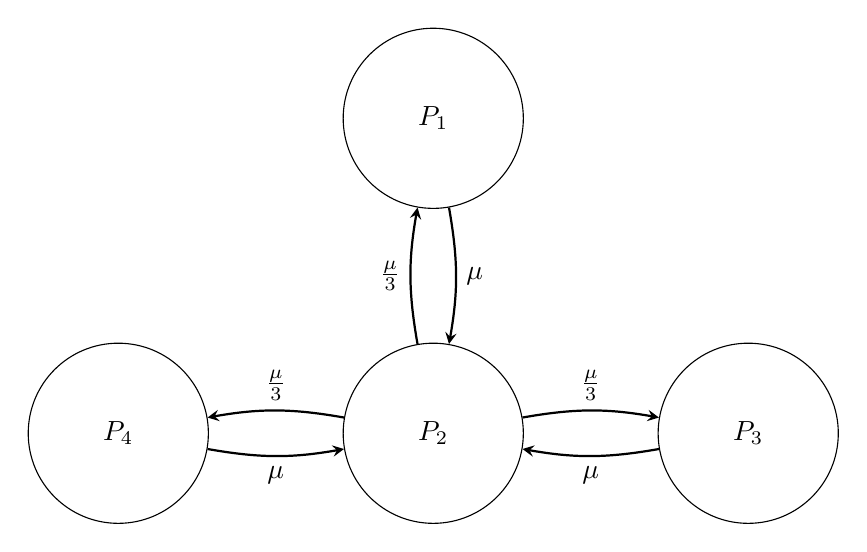
\begin{tikzpicture}[node distance = 4cm]
        \node (popone) [member] {$P_1$}    ;
        \node (poptwo) [member, below of = popone] {$P_2$}    ;
        \node (popthree) [member, right of = poptwo] {$P_3$}  ;
        \node (popfour) [member, left of = poptwo] {$P_4$}    ;
        
        \draw [arrow] (popone) to [out = -80, in = 80] node[anchor = west]{$\mu$} (poptwo);
        \draw [arrow] (poptwo) to [out = 100, in = -100] node[anchor = east]{$\frac{\mu}{3}$} (popone);
        \draw [arrow] (poptwo) to [out = 10, in = 170] node[anchor = south]{$\frac{\mu}{3}$} (popthree);
        \draw [arrow] (popthree) to [out = -170, in = -10] node[anchor = north]{$\mu$} (poptwo);
        \draw [arrow] (poptwo) to [out = 170, in = 10] node[anchor = south]{$\frac{\mu}{3}$} (popfour);
        \draw [arrow] (popfour) to [out = -10, in = -170] node[anchor = north]{$\mu$} (poptwo);
        
    \end{tikzpicture}
    \caption{}
    \label{fig:my_label}
\end{subfigure}


\caption{(a) A schematic model of population change due to the white-nose syndrome (WNS) in a bat population where $S$ represents the proportion of the population susceptible to WNS, $E$ the proportion exposed to WNS but not symptomatic, $I_1$ the proportion infected for 1 year, and $I_2$ the proportion of bats infected for at least 2 years. Further parameters are as defined in Table 1. (b) A schematic model of the metapopulation. The populations are arranged in a spider arrangement such that only individuals in the population $P_2$ may migrate to any of the other populations directly. The individuals migrate at an annual rate $\mu$. Since inidividuals of $P_2$ may migrate to any of the other populations, we assume an equal chance of migrating to each of those populations, $\frac{\mu}{3}$.}
 
\end{figure}
    
    
    

\section*{\centering \sc \large Results}
 
 \subsection*{\sc\textit{Parameter Estimation and Sensitivity Analyses}}
 
 Table 1 lists a  summary of all the parameters involved and their estimates. We relied on previous studies to extract and estimate most of the parameters. Since we looked at the annual change in proportion of populations, some of the parameter values were estimated from daily values used by Meyer et al. (2016). For instance, the annual rate of progression from exposed to infected bats was estimated multiplying the known default value by 365 days/year ($\tau = 1/83 d^{-1} \times 365 d. y^{-1} = 365/83 y^{-1}$). 
 
\begin{table}
\def\tabularxcolumn#1{m{#1}}
\newcolumntype{Q}{>{\arraybackslash}>{\hsize=6cm}X}
\newcolumntype{P}{>{\arraybackslash}>{\hsize=4cm}X}
\begin{tabularx}{\textwidth}{l Q l l P}
        \hline
        Symbol  &   Description & Units &  Value & Notes\\\hline
        \beta   &   Transmissive contact between susceptible and exposed and infected bats & $y^{-1}$ & $0-766.5$ & estimated  from Meyer \textit{et al.} (2016)\\
        \tau    &   Annual rate of progression from exposed to infectious & $y^{-1}$ & $365/83$ & (Meyer \textit{et al.}, 2016; Lorch \textit{et al.} 2011)\\
        \gamma & Annual rate of bat maturation & $y^{-1}$ & 0.762 & average of rates for males and females from Keen \& Hitchcock(1980)\\
        $a_1$ & the probability of recovery of exposed bats and bats infected for under one year & unitless & 0.75 & (Meyer \textit{et al.} 2016)\\
        $a_2$ & the probability of recovery of bats infected for at least two yeasr & unitless & $1/11$ & (Meyer \textit{et al.} 2016)\\
        $m_1$ & mortality of bats infected for one year & $y^{-1}$ & 0.20 & (Frick \textit{et al.} 2010)\\
        $m_2$ & mortality of bats infected for at least two years & $y^{-1}$ & 0.70 & (Frick \textit{et al.} 2010)\\
        $\mu$ & annual migration rate between populations & $y^{-1}$& 0.04 & (Norquay \textit{et al.} 2013) \\\hline
        
\end{tabularx}
\caption{Summary of known parameter values and estimates for the model from previous literature. Some of these values have been estimated from daily rates during the hibernation phase.}
\end{table}
 
We performed sensitivity analyses for the transmissive contact rate between bats, $\beta$,  and the migration rates between populations, $\mu$. Looking at the changes in the population dynamics with increasing transmissive contact rate, we see that there is always an immediate increase in the proportion of individuals exposed to WNS and the proportion of susceptible individuals declines rapidly. Even at a lower contact rate ($\beta = 100$) , the proportion of individuals exposed quickly rises up to 70\% of the population. At contact rates higher in the range estimated by Meyer et al. (2016), the proportion of individuals exposed quickly rises up to more than 95\% of the population (Fig. 2). On the other hand, we performed a sensitivity analysis for the migration over the range of 0-0.10. With increasing migration rate between equal sized populations, we see that all the populations are exposed to WNS rapidly and show similar dynamics. However, there is a slight delay in the commencement of these dynamics indicating the period when the disease is not prevalent in the population but this is rather short. Figure 3 shows the population dynamics for a migration rate $\mu = 0.04$ between equal sized populations. For the population viability analyses, we fix the value to migration rate between colonies based on previous studies (Norquay \textit{et al.} 2013). 

\begin{figure}
    \centering
    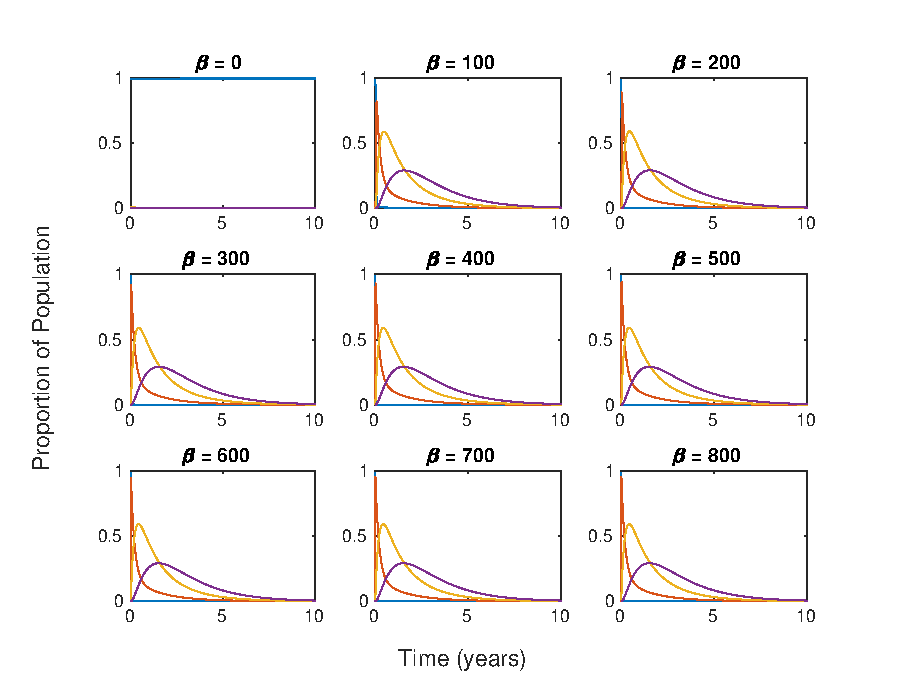
\includegraphics{sens_beta.eps}
    \caption{Sensitivity analysis of the transmissive contact rate between bats. As the transmissive contact rate increases, the maximum  proportion of individuals exposed to WNS also increases. Legend: Susceptible - blue, exposed - red, infected for 1 year - orange, and infected for at least 2 years purple. }
    \label{fig:my_label}
\end{figure}



\subsection*{\sc\textit{Population Viability Analyses}}

We look at the difference in size of populations and the dynamics of white-nose syndrome. When the initial population sizes are equal, all populations show similar dynamics except for a slight delay in the populations where the disease is introduced (Fig. 3). However, we see all the populations decline before 10 years. When the initial infected population is larger than other populations (Fig. 4(a)), including an empty one, the populations decline rapidly. In the newly occupied population 4, we see that the proportion of susceptible individuals stabilizes and that of infected bats decreases. However, this proportion of susceptible is around 0.001 of the whole metapopulation. Similarly, when the initial infected population is smaller (Fig. 4 (b)), the total metapopulation declines rapidly but the newly occupied population stabilizies. However, in this case, it is much lower than when the initial infected population was larger and stabilizes at about $7.5 \times 10^{-4}$. Furthermore, the difference in population proportion of initial infected population does not seem to change the rate of decline of the metapopulation. 

\begin{figure}
    \centering
    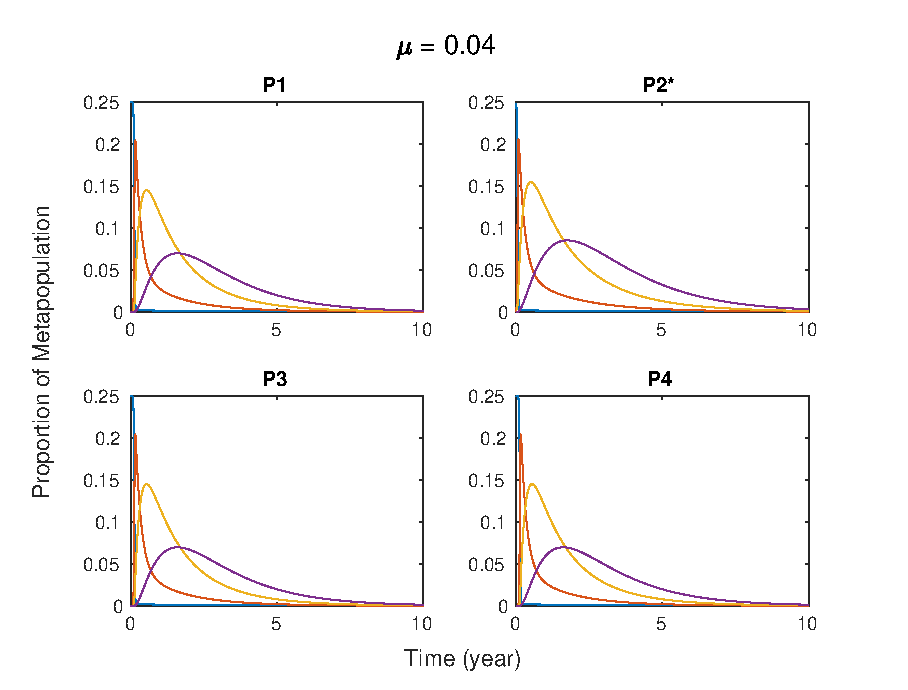
\includegraphics{mu_5.eps}
    \caption{The population dynamics for a fixed migration rate for equal sized initial populations.  Legend: Susceptible - blue, exposed - red, infected for 1 year - orange, and infected for at least 2 years purple.}
    \label{fig:my_label}
\end{figure}

\begin{figure}
    \centering
    \begin{subfigure}{\textwidth}
    \centering
    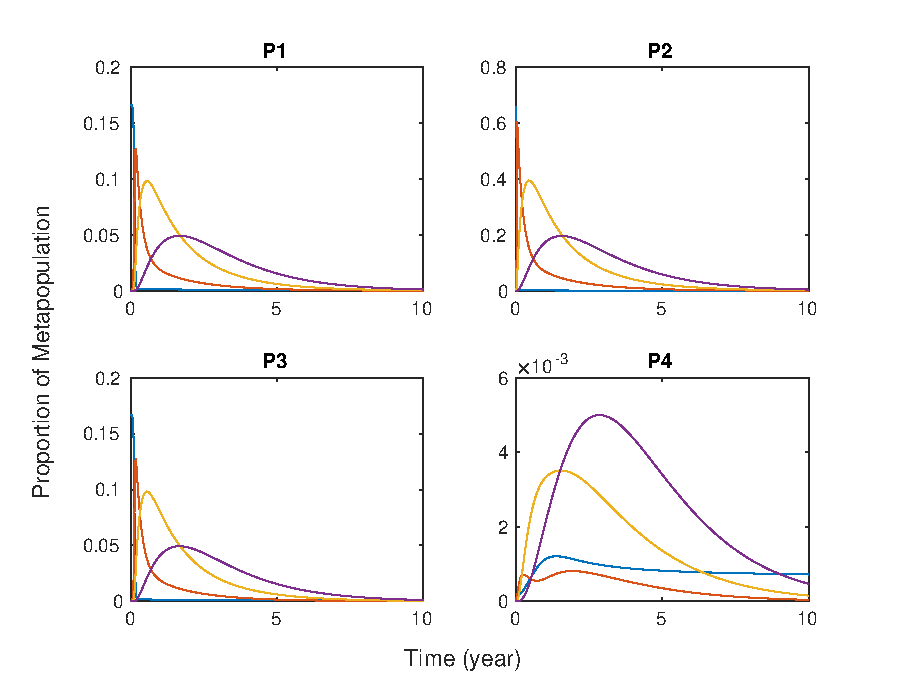
\includegraphics[width = 0.75\textwidth]{large_pop.eps}
    \caption{}
    \end{subfigure}
    \begin{subfigure}{\textwidth}
    \centering
    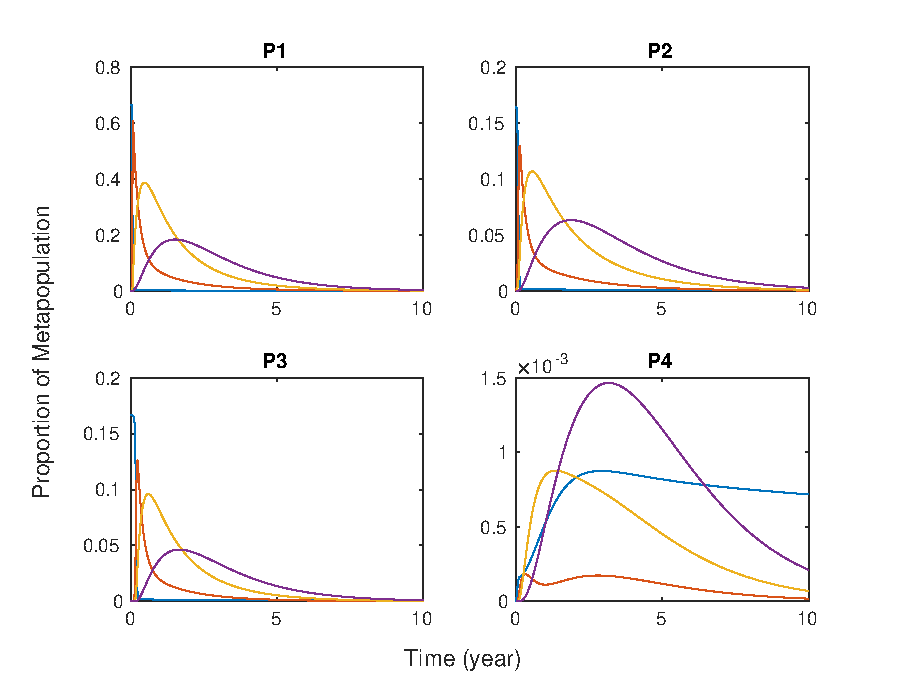
\includegraphics[width = 0.75\textwidth]{small_pop.eps}
    \caption{}
    \end{subfigure}
    \caption{Population viability for (a) when the initial infected population (P2) is larger than the other populations and one population is not occupied, (b) when the initial infected population (P2) is smaller than another population and one population is not occupied.  Legend: Susceptible - blue, exposed - red, infected for 1 year - orange, and infected for at least 2 years purple.}
    \label{fig:my_label}
\end{figure}


\section*{\centering \sc \large Discussion}

From our som our simulations of fungus transmittance through 4 little brown bats subpopulations through a timescale of 10 years, regardless of starting total population size prior to infection, it was observed that the mortality from the fungus would be completely eradicating the little brown bat total population before 10 years, without taking into consideration of natural mortality yet. This observation would be of high concern since the little brown bat average life span is around 6 – 10 years, showing that if conservative actions are not implemented quickly, it may be too late for a lot of the little brown bat populations in North America. While we did predict if the original little brown bat total population was above a certain size before infection by P.destructans, logically, the population may persist, but unfortunately P.destructans’s hazard rate is stated to nearly “double for each ten-fold increase of hibernating bats in a colony” (Wilder, 2011) so increasing the initial population size prior to fungal infection to a “critical threshold” would not be able to alleviate the destructive effects toward the little brown bat population.
 
From the sensitivity analysis of the contact rate and rates of bats migration within different caves, it is observed that contact rates between bats have the largest impact on transmitting the fungus across the total bat population, compared to migratory rates. While it is almost impossible to control the rates of bats coming into contact with another bat, especially during mating seasons, and that P.destructans does not show density-dependence transmittance in colonies that roost in dense clusters like the little brown bat (Langwig, 2012) it is slightly reassuring that bats infected with P.destructans were observed to roost solitarily away from large hibernacula (Wilcox, 2014), a behaviour that may reduce the chance of P.destructans being present in a cave populated with a huge population of bats, hence reducing contact rate indirectly, at the expense of the infected individual’s life since it would not have the additional heat from the dense packing of hibernating bat to help it maintain a stable body temperature to survive through the winters.       

Although our model was constructed to try to replicate the intrapopulation host-parasite infection dynamics of P.destructans in an infected population of little brown bats as closely to actual observed mortality rates in literature, it did not include other factors that may help describe the host-parasite interactions dynamics in better details. In our model, the main factors that may help understand the rate of fungal transmission between bat populations that were not taken into consideration were the sex ratios of migrants flying away from a cave, persistence of P.destructans in the cave environment outside of the body of the little brown bat, and possible host resistance to the fungus. 
For sex ratios, it was observed that young male bats would often leave their birth cave and rarely return while young female bats are more likely to remain in the cave of their birth for most of their lives (Smith, 1957). This observation could lead to a hypothesis that young male bats could be the main vector for fungal transmission between distant caves.

A factor that may impact how the P. destructans interact with bats is the fungal ability to persist on the walls of caves independently. P. destructans was observed to be able to persist for 1-2 years after exclusion of an entire bat population in a cave (Lorch, 2013), signifying that it is able to persist for quite a long time. This persistence in the external abiotic environment would affect the transmission rate of the fungus to bat hosts, as it could infect bats when they fly into an infective cave to roost without the need of contact through an infected bat but through direct contact with fungal spores on the walls of the cave, leading to caves to be viewed as environmental reservoirs for P. destructans (Frick, 2016).  

While our model was not able to show the strength of other factors that may also impact transmission of the fungi within a population of bats, other than migratory rates and contact rates, it was able to highlight the significance of migratory rates for the fungi to travel long distances across distant caves due to its host migratory patterns, a phenomena that has been observed with P. destructans presence in North America, where it has begun to show a directional movement westward across the continent. (Maher, 2012) While our model lacks information to determine the average rate of how fast P. destructans is moving across North America, future studies should be held on the social behaviours, particularly the migratory patterns of bats that would be the most resistant to the fungus, as they may act involuntarily as vectors to transmit the fungus to populations that would be of a higher risk. Since P. destructans is a generalistic pathogen, understanding of its rate of spread could allow conservationists to design protocols targeting the migratory patterns of the host bats to reduce the spread of P. destructans across a nation as much as possible, and if possible, may allow local containment of the fungus within a designated area of surveillance, for example restrict the presence of the fungus to only a small group of isolated caves away from the majority of the bat populations main winter roosting sites in North America.  

Perspectives on possible conservation efforts to help the little brown bat populations mitigate the detrimental effects of P. destructans have been mixed. On one case, in the article “Observed Resiliency of Little Brown Myotis to Long-Term White-Nose Syndrome Exposure”, researcher C. A. Dobony (2018) claims that since little brown bats that are infected with white-nose syndrome are capable of persisting in the absence of human intervention, minimal human intervention is required since there are signs that the population is evolving a natural resistance (Dobony, 2018). On another case, in Palmer et al. (2018) discovered that P. destructans lacks a “key enzyme, UVE1” in its alternative excision repair pathway allowing it to be susceptible to DNA damage from UV radiation, specifically treatment with UV-C light. This has lead to the proposal of future studies to “understand the physiological effect of UV-C light on bats” with the intention to treat bats infected with P. destructans with UV-C light. (Palmer, 2018) Unfortunately, due to lack of information, it is unsure how the bats would react to the presence of a UV-C light source in their roosting sites. 

Our proposal toward conservation efforts for the little brown bat would be more focused on the concept of caves as long-term environmental reservoirs (Hoyt, 2015). Since P. destructans has an upper critical temperature for possible growth of around 20 degrees Celsius (Verant, 2016), more studies about the microclimate of caves should be performed to see if it would be possible to raise the overall temperature inside the cave above $20^0$C to inhibit the growth of P. destructans as much as possible. The other proposals are less far-fetched as the temperature proposal, and involves researcher C. A. Dobony’s (2018) perspective of minimizing human contact with already-identified-to-be-infected populations of bats. Spores of P. destructans were found to be able to persist on human clothing in cold temperatures (Hoyt, 2015), so humans may indirectly act as a vector for P. destructans between caves..



\section*{\centering \sc \large References}

\parindent -0.5cm \hangindent=0.5cm Arias-Cóyotl, E., Stoner, K., \& Casas, A. (2006). Effectiveness of Bats as Pollinators of Stenocereus stellatus (Cactaceae) in Wild, Managed In situ, and Cultivated Populations in La Mixteca Baja, Central Mexico. American Journal of Botany, 93(11), 1675-1683.
 
\hangindent=0.5cm Beekman CN, Meckler L, Kim E, Bennett RJ (2018) Galleria mellonella as an insect model for P. destructans, the cause of White-nose Syndrome in bats
 
\hangindent=0.5cm Blehert, D., Hicks, A., Behr, M., Meteyer, C., Berlowski-Zier, B., Buckles, E., . . . Stone, W. (2009). Bat White-Nose Syndrome: An Emerging Fungal Pathogen? Science, 323(5911), new series, 227-227.
 
\hangindent=0.5cm Dobony, C. A., \& Johnson, J. B. (2018). Observed Resiliency of Little Brown Myotis to Long-Term White-Nose Syndrome Exposure. Journal of Fish and Wildlife Management, 9(1), 168-179.
 
\hangindent=0.5cm Dubois, J. E., \& Monson, K. M. (2007). Recent Distribution Records of the Little Brown Bat, Myotis lucifugus, in Manitoba and Northwestern Ontario. The Canadian Field-Naturalist, 121(1), 57.
\hangindent=0.5cm Frick, W. F., J. F. Pollock, A. C. Hicks, K. E. Langwig, D. S. Reynolds, G. G. Turner, C. M. Butchkoski, and T. H. Kunz. 2010a. An emerging disease causes regional population collapse of a common North American bat species. Science 329(5992): 679-682.

\hangindent=0.5cm Frick, W. F., Puechmaille, S. J., \& Willis, C. K. (2016). White-nose syndrome in bats. In Bats in the Anthropocene: Conservation of bats in a changing world (pp. 245-262). Springer, Cham.
 
\hangindent=0.5cm Hanski, I. (1998), Metapopulation dynamics. Nature, 396: 41-49.
 
\hangindent=0.5cm Hoyt, J. R., Langwig, K. E., Okoniewski, J., Frick, W. F., Stone, W. B., \& Kilpatrick, A. M. (2015). Long-term persistence of Pseudogymnoascus destructans, the causative agent of white-nose syndrome, in the absence of bats. EcoHealth, 12(2), 330-333.
 
\hangindent=0.5cm Ivar Vleut, Samuel I. Levy-Tacher, Jorge Galindo-González, Willem F. de Boer. 2015. Positive effects of surrounding rainforest on composition, diversity and late-successional seed dispersal by bats. Basic and Applied Ecology. 16:308-315

\hangindent=0.5cm Keen, R. & Hitchcock, H. (1980). Survival and Longevity of the Little Brown Bat (Myotis lucifugus) in Southeastern Ontario. Journal of Mammology, 60(1):1-7.


\hangindent=0.5cm Langwig KE, Frick WF, Bried JT, Hicks AC, Kunz TH, Kilpatrick AM (2012) Sociality, density-dependence and microclimates determine the persistence of populations suffering from a novel fungal disease, white-nose syndrome. Ecol Lett 15:1050–1057
 
\hangindent=0.5cm Langwig, K. E., Hoyt, J. R., Parise, K. L., Frick, W. F., Foster, J. T., & Kilpatrick, A. M. (2017). Resistance in persisting bat populations after white-nose syndrome invasion. Philosophical Transactions of the Royal Society B: Biological Sciences, 372(1712), 20160044.
 
\hangindent=0.5cm Lorch, J., Lindner, D., Gargas, A., Muller, L., Minnis, A., & Blehert, D. (2013). A culture-based survey of fungi in soil from bat hibernacula in the eastern United States and its implications for detection of Geomyces destructans, the causal agent of bat white-nose syndrome. Mycologia, 105(2), 237-252.

\hangindent=0.5cm Lorch, J. M., Muller, L. K., Russell, R. E., O'Connor, M., Lindner, D. L., & Blehert, D. S. (2013). Distribution and environmental persistence of the causative agent of white-nose syndrome, Geomyces destructans, in bat hibernacula of the eastern United States. Appl. Environ. Microbiol., 79(4), 1293-1301.
 
\hangindent=0.5cm Maher, S. P., Kramer, A. M., Pulliam, J. T., Zokan, M. A., Bowden, S. E., Barton, H. D., ... & Drake, J. M. (2012). Spread of white-nose syndrome on a network regulated by geography and climate. Nature communications, 3, 1306.

\hangindent= 0.5cm Meyer, A.D., Stevens, D.F., & Blackwood, J.C. (2016). Predicting bat colony survival under controls targeting multiple transmission routes of white-nose syndrome. Journal of Theoretical Biology 409: 60-69.
 
\hangindent=0.5cm Palmer, J. M., Drees, K. P., Foster, J. T., & Lindner, D. L. (2018). Extreme sensitivity to ultraviolet light in the fungal pathogen causing white-nose syndrome of bats. Nature communications, 9(1), 35.
 
 
\hangindent=0.5cm Norquay, K. J. O., F. Martinez-Nunez, J. E. Dubois, K. M. Monson, and C. K. R. Willis. 2013. Long-distance movements of little brown bats (Myotis lucifugus). Journal of Mammalogy 94(2): 506-515.
 
\hangindent=0.5cm Smith, E. (1957). Experimental study of factors affecting sex ratios in the little brown bat. Journal of Mammalogy, 38(1), 32-39.
 
\hangindent=0.5cm Verant, M. L., Boyles, J. G., Waldrep Jr, W., Wibbelt, G., & Blehert, D. S. (2012). Temperature-dependent growth of Geomyces destructans, the fungus that causes bat white-nose syndrome. PloS one, 7(9), e46280.
 
\hangindent=0.5cm Wilcox, A., Warnecke, L., Turner, J. M., McGuire, L. P., Jameson, J. W., Misra, V., ... & Willis, C. K. (2014). Behaviour of hibernating little brown bats experimentally inoculated with the pathogen that causes white-nose syndrome. Animal Behaviour, 88, 157-164.

\hangindent=0.5cm Wilder, A. P., Frick, W. F., Langwig, K. E., & Kunz, T. H. (2011). Risk factors associated with mortality from white-nose syndrome among hibernating bat colonies. Biology Letters, 7(6), 950-953.

    





\end{document}




















